\section {Foundations of dataflow analysis}
\setlength{\parindent}{0pt}
(Prepared by Vardhan Jain)

\vspace{0.3cm}

\subsection{Advantages of common Dataflow Analysis framework}
\begin{itemize}
    \item \textbf{Prove properties for an entire family of problems} : We prove properties for the framework
    and basically we have proven properties for different dataflow analysis problems together.
    \item \textbf{Aids in software engineering} : We can write the basic logic in a base class and all our data 
    flow analysis algorithms can be derived from that base class. We won't have to repeat the same logic.
\end{itemize}

\subsection{Dataflow Analysis problems \textbf{($F$, $V$, \^{})} are defined by}
\begin{itemize}
    \item \textbf{A semilattice ($V$, \^{})} : Semilattice is defined by the domain of values represented by $V$ and
    the meet operator \^{} represented by the caret symbol.
    \item \textbf{A family of transfer functions $F:V\rightarrow V$} : A transfer function is defined as a function that takes value 
    from the set of values $V$ and returns value in the same set of values $V$. $F$ represents family of all such possible functions.
    They need to satisfy certain properties in order to be admissible.
\end{itemize}
\subsection{Semilattice}
A semilattice S = \textless a set of values $V$, a meet operator \^{} where the meet operator \^{} \textgreater  has the following properties:
\begin{itemize}
    \item \textbf{Idempotent} x \^{} x = x
    \item \textbf{Commutative} x \^{} y = y \^{} x
    \item \textbf{Associative}  x \^{} (y \^{} z) = (x \^{} y) \^{} z
\end{itemize}
Examples of meet operator \^{} - set-union, set-intersection, and, or, min, max \\
Some non-examples of meet operator are add, subtract, multiply, divide etc.

\subsection{Semilattice example}
V = \{x {\textbar} x is the subset of \{$d_{1}$, $d_{2}$, $d_{3}$\}\}, \^{} $\triangleq$ set-union, 
Ordering $\leq$ $\triangleq$ $\supseteq$. Figure \ref{fig:semilattice_union} shows the semilattice diagram, the nodes represent the values and the edge represent the ordering. If there is an edge from a to b then a $\geq$ b. More precisely there is a path from node a to node b iff a $\geq$ b. This is a partial ordering as not all values are comparable. Meet of two values $v_{1}$ and $v_{2}$ can be inferred from the semilattice diagram as the first common descendant node of nodes with values $v_{1}$ and $v_{2}$.\par
Another example contains values as 2-tuples booleans. The four possible values are \{true, true\}, \{false, true\}, \{true, false\} and \{false, false\}. The semilattice diagram is shown in figure \ref{fig:semilattice_and}. Here \^{} is logical AND.
\begin{figure}
    \centering
    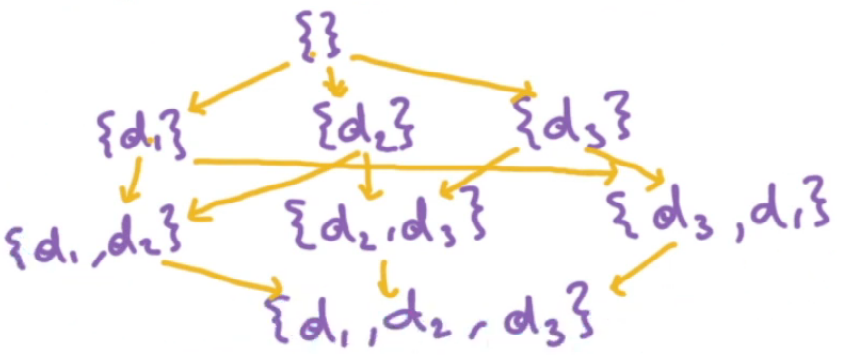
\includegraphics[width=1\linewidth]{images/semilatticeSetUnion.png}
    \caption{Set union semilattice example}
    \label{fig:semilattice_union}
\end{figure}
\begin{figure}[h!]
\caption{Boolean tuples logical AND semilattice example}
\begin{center}
\begin{tikzpicture}[-latex ,auto ,node distance =3.5cm and 5cm ,on grid ,
    semithick ,
    state/.style ={ rectangle ,top color =white , bottom color = blue!20 ,
    draw, blue , text=blue , scale = 0.7 ,minimum width =3.5 cm, minimum height = 1.5 cm}]
    \node[state] (A){} node [label = {[label distance = 0.55cm]90:Block A}, rectangle split,rectangle split parts=2]{%
      \{true, true\}%
      };
    \node[state] (B) [below left = of A]{} node [label = {[label distance = 0.55cm]90:Block B},rectangle split,rectangle split parts=2] [below left = of A] {%
      \{false, true\}%
      };
    \node[state] (D) [below right =of A]{} node [label = {[label distance = 0.55cm]90:Block C},rectangle split,rectangle split parts=2] [below right = of A] {%
      \{true, false\}%
      };
    \node[state] (E) [below left =of D]{} node [label = {[label distance = 0.55cm]90:Block D},rectangle split,rectangle split parts=2] [below left = of D] {%
      \{false, false\}%
      };
    \path[->] (A) edge node [above = 0.3 cm] {} (D);
    \path[->] (A) edge node [above = 0.3 cm] {} (B);
    \path[->] (B) edge  (E);
    \path[->] (D) edge  (E);
    
\end{tikzpicture}
\end{center}
\label{fig:semilattice_and}
\end{figure}

\subsection{Semilattice properties}
\begin{itemize}
    \item x \^{} y is the first common descendant of x and y.
    \item Define top value T such that x \^{} T = x for all x
    \item Define bottom ($\bot$) such that x \^{} $\bot$ = $\bot$ for all x
    \item Semilattice diagram = picture of partial orders
    
\end{itemize}



% \subsection{Example of \^{} and $\leq$}
% Set-union